%% Scientific Conference Poster Template
%% tikzposter class | Portrait A0 | 2-column layout
%% Portrait orientation: standard for most scientific conferences
%% For ICML/CVPR landscape, change "portrait" to "landscape" and use 3 columns
%% Compile with: pdflatex poster.tex
%%
%% Design principles:
%%   - Portrait A0 (841mm x 1189mm), most common conference format
%%   - 2-column layout, read down left then down right
%%   - Minimal text (~500 words), maximum visual impact
%%   - tikzfigure environments (NOT standard figure) to prevent overflow
%%   - Relative sizing (linewidth-based) for all figures/charts
%%   - Generous padding (15mm+) to prevent content-edge collisions

\documentclass[25pt, a0paper, portrait, margin=15mm,
    innermargin=15mm, blockverticalspace=12mm, colspace=20mm]{tikzposter}

% Packages
\usepackage[utf8]{inputenc}
\usepackage[T1]{fontenc}
\usepackage{amsmath, amssymb}
\usepackage{graphicx}
\usepackage{booktabs}
\usepackage{enumitem}
\usepackage{pgfplots}
\pgfplotsset{compat=1.18}
\usepackage{qrcode}

% Use sans-serif for better poster readability at distance
\renewcommand{\familydefault}{\sfdefault}

% ===== COLOR SCHEME (Navy + White + Amber accent) =====
% High contrast, professional, stands out at conferences
% --- Alternative schemes (uncomment ONE set, comment out the active set) ---
%% Forest Green (biology/environmental):
%   \definecolor{navyblue}{HTML}{166534} \definecolor{steelblue}{HTML}{4ADE80}
%   \definecolor{amber}{HTML}{92400E} \definecolor{darktext}{HTML}{1C1917}
%   \definecolor{lightbg}{HTML}{F0FDF4}
%% Medical Teal (healthcare/clinical):
%   \definecolor{navyblue}{HTML}{0F766E} \definecolor{steelblue}{HTML}{5EEAD4}
%   \definecolor{amber}{HTML}{F43F5E} \definecolor{darktext}{HTML}{1E293B}
%   \definecolor{lightbg}{HTML}{F0FDFA}
%% Tech Purple (CS/ML/AI):
%   \definecolor{navyblue}{HTML}{6D28D9} \definecolor{steelblue}{HTML}{A78BFA}
%   \definecolor{amber}{HTML}{EC4899} \definecolor{darktext}{HTML}{1E1B4B}
%   \definecolor{lightbg}{HTML}{FAF5FF}
%% Minimal Dark (high contrast/modern):
%   \definecolor{navyblue}{HTML}{1F2937} \definecolor{steelblue}{HTML}{6B7280}
%   \definecolor{amber}{HTML}{DC2626} \definecolor{darktext}{HTML}{111827}
%   \definecolor{lightbg}{HTML}{F9FAFB}
% --- Active scheme (Navy + Amber) ---
\definecolor{navyblue}{HTML}{1E3A8A}
\definecolor{steelblue}{HTML}{3B82F6}
\definecolor{amber}{HTML}{F59E0B}
\definecolor{darktext}{HTML}{1F2937}
\definecolor{lightbg}{HTML}{F8FAFC}

% ===== CUSTOM TITLE STYLE =====
\definetitlestyle{ConferenceTitle}{
    width=\paperwidth, roundedcorners=0, linewidth=0pt, innersep=2cm,
    titletotopverticalspace=0mm, titletoblockverticalspace=20mm
}{
    \begin{scope}[line width=\titlelinewidth, rounded corners=\titleroundedcorners]
        \fill[color=navyblue] (\titleposleft,\titleposbottom) rectangle (\titleposright,\titlepostop);
        % Accent bar at bottom of title
        \fill[color=amber] (\titleposleft,\titleposbottom) rectangle (\titleposright,\titleposbottom+0.5cm);
    \end{scope}
}

% ===== CUSTOM BLOCK STYLE =====
\defineblockstyle{ConferenceBlock}{
    titlewidthscale=1, bodywidthscale=1, titleleft,
    titleoffsetx=0pt, titleoffsety=0pt, bodyoffsetx=0pt, bodyoffsety=0pt,
    bodyverticalshift=0pt, roundedcorners=8, linewidth=2pt,
    titleinnersep=10mm, bodyinnersep=15mm
}{
    \draw[color=steelblue!40, fill=white, rounded corners=\blockroundedcorners, line width=1pt]
        (blockbody.south west) rectangle (blockbody.north east);
    \ifBlockHasTitle
        \draw[color=navyblue, fill=navyblue, rounded corners=\blockroundedcorners]
            (blocktitle.south west) rectangle (blocktitle.north east);
    \fi
}

% Apply styles
\usetheme{Default}
\usetitlestyle{ConferenceTitle}
\useblockstyle{ConferenceBlock}

% Set colors
\colorlet{backgroundcolor}{white}
\colorlet{framecolor}{steelblue}
\colorlet{titlebgcolor}{navyblue}
\colorlet{titlefgcolor}{white}
\colorlet{blocktitlebgcolor}{navyblue}
\colorlet{blocktitlefgcolor}{white}
\colorlet{blockbodybgcolor}{white}
\colorlet{blockbodyfgcolor}{darktext}

% Remove tikzposter watermark
\tikzposterlatexaffectionproofoff

% ===== TITLE CONTENT =====
% CUSTOMIZATION: Replace with your details
\title{\parbox{0.90\linewidth}{\centering\textbf{%
    Efficient Neural Architecture Search via\\[0.2em]
    Gradient-Based Optimization with Adaptive Resource Allocation}}}
\author{Alice Chen$^{1}$, Bob Kumar$^{2}$, Carol Zhang$^{1}$, David Patel$^{3}$}
\institute{$^{1}$Department of Computer Science, Stanford University \quad
           $^{2}$Google DeepMind \quad
           $^{3}$MIT CSAIL \\[0.3em]
           \texttt{achen@stanford.edu} \quad
           \texttt{github.com/achen/enas-adaptive}}

\begin{document}

\maketitle

% ===== 2-COLUMN LAYOUT (50% / 50%) =====
% Portrait poster: read down left column, then down right column
\begin{columns}

    % ============================================================
    % LEFT COLUMN: Motivation, Methods, Setup
    % ============================================================
    \column{0.50}

    \block{Motivation}{
        Neural Architecture Search (NAS) automates the design of neural networks, but existing methods face two critical limitations:

        \vspace{1em}
        \begin{itemize}[leftmargin=*, itemsep=0.8em]
            \item \textbf{Computational cost:} Current methods require $10^3$--$10^4$ GPU hours
            \item \textbf{Resource allocation:} Fixed budgets waste computation on unpromising architectures
        \end{itemize}

        \vspace{1em}
        \coloredbox[bgcolor=amber!15, fgcolor=darktext, roundedcorners=5] while improving final accuracy.
        }
    }

    \block{Method: ENAS-Adaptive}{
        Our approach combines three components:

        \vspace{1em}
        % Workflow diagram -- uses center + tikzpicture (NOT figure env)
        \begin{center}
        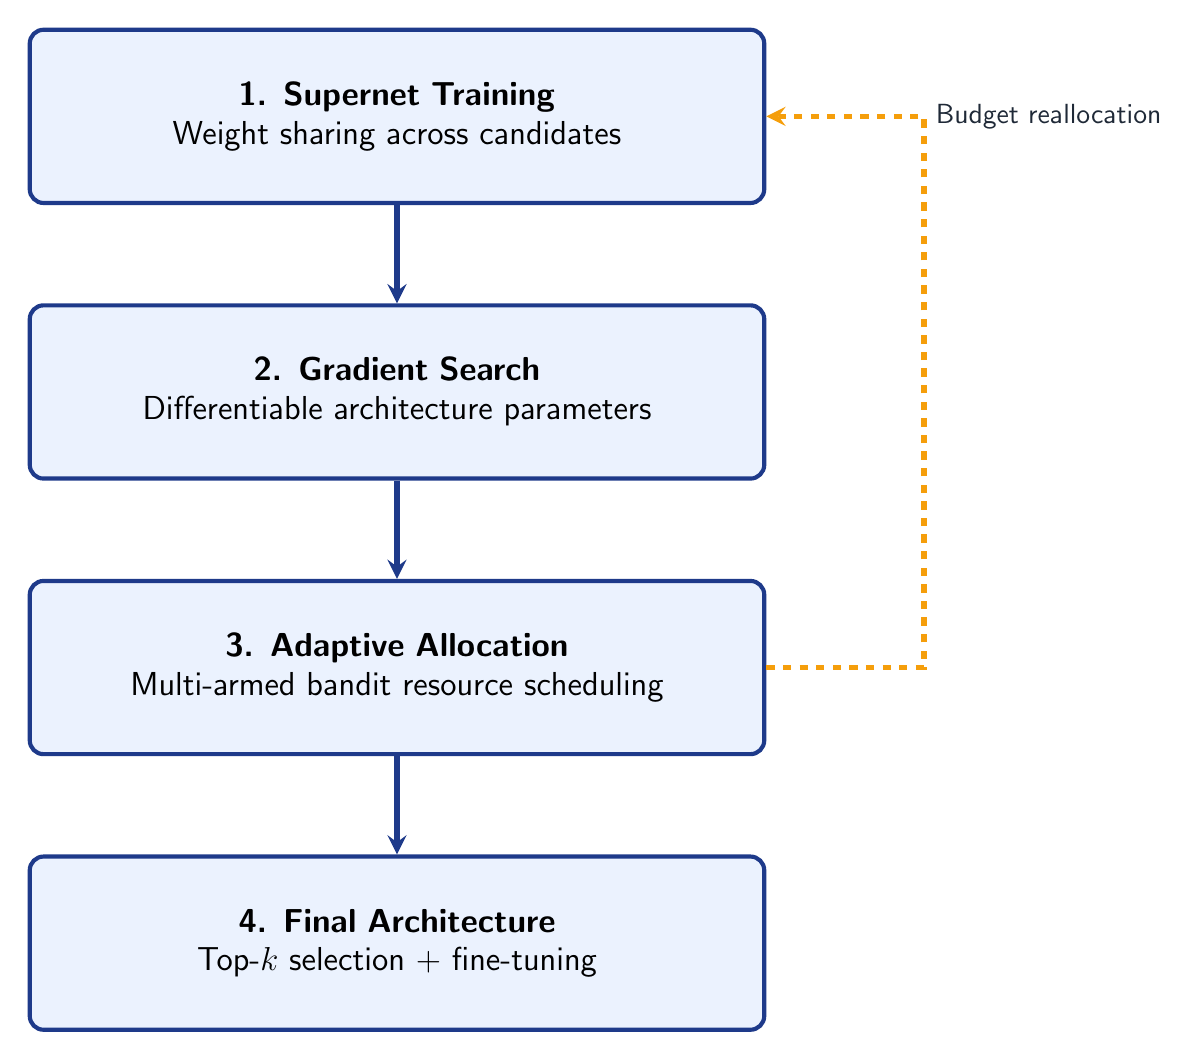
\begin{tikzpicture}[
            node distance=3.5cm,
            box/.style={rectangle, draw=navyblue, fill=steelblue!10,
                        text width=0.75\linewidth, text centered, rounded corners=5pt,
                        minimum height=2.2cm, line width=1.5pt, font=\large},
            arrow/.style={->, >=stealth, line width=2pt, color=navyblue}
        ]
            \node[box] (supernet) {\textbf{1. Supernet Training}\\Weight sharing across candidates};
            \node[box, below of=supernet] (search) {\textbf{2. Gradient Search}\\Differentiable architecture parameters};
            \node[box, below of=search] (allocate) {\textbf{3. Adaptive Allocation}\\Multi-armed bandit resource scheduling};
            \node[box, below of=allocate] (output) {\textbf{4. Final Architecture}\\Top-$k$ selection + fine-tuning};

            \draw[arrow] (supernet) -- (search);
            \draw[arrow] (search) -- (allocate);
            \draw[arrow] (allocate) -- (output);

            % Feedback loop
            \draw[arrow, dashed, color=amber] (allocate.east) -- ++(2cm,0) |- (supernet.east)
                node[midway, right, font=\normalsize, text=darktext] {Budget reallocation};
        \end{tikzpicture}
        \end{center}

        \vspace{1em}
        \textbf{Adaptive allocation} uses Thompson sampling to dynamically redistribute GPU hours from low-performing candidates to promising ones during search.
    }

    \block{Datasets \& Setup}{
        \vspace{0.5em}
        \begin{center}
        {\large
        \begin{tabular}{lcc}
            \toprule
            \textbf{Dataset} & \textbf{Train/Val/Test} & \textbf{Classes} \\
            \midrule
            CIFAR-10     & 45K / 5K / 10K  & 10  \\
            CIFAR-100    & 45K / 5K / 10K  & 100 \\
            ImageNet-1K  & 1.2M / 50K / -- & 1000 \\
            \bottomrule
        \end{tabular}
        }
        \end{center}

        \vspace{1em}
        Search conducted on CIFAR-10; best architecture transferred to CIFAR-100 and ImageNet. All experiments on 8$\times$ NVIDIA A100 GPUs.
    }

    \block{Ablation Study}{
        \vspace{0.5em}
        \begin{center}
        {\large
        \begin{tabular}{lcc}
            \toprule
            \textbf{Configuration} & \textbf{Acc.} & \textbf{Hours} \\
            \midrule
            Full model (ours)         & \textbf{97.82\%} & \textbf{0.4} \\
            \quad w/o adaptive alloc.  & 97.41\%           & 1.1           \\
            \quad w/o gradient search  & 96.88\%           & 3.2           \\
            \quad w/o weight sharing   & 97.35\%           & 8.7           \\
            \bottomrule
        \end{tabular}
        }
        \end{center}

        \vspace{1em}
        Each component contributes meaningfully:
        \begin{itemize}[leftmargin=*, itemsep=0.5em]
            \item Adaptive allocation: +0.41\% accuracy, 2.75$\times$ speedup
            \item Gradient search: +0.94\% accuracy, 8$\times$ speedup
            \item Weight sharing: +0.47\% accuracy, 21.75$\times$ speedup
        \end{itemize}
    }


    % ============================================================
    % RIGHT COLUMN: Results, Analysis, Conclusions
    % ============================================================
    \column{0.50}

    \block{Main Results}{
        % Bar chart -- relative width prevents overflow
        \begin{tikzfigure}[Accuracy vs.\ search cost across NAS methods on CIFAR-10]
            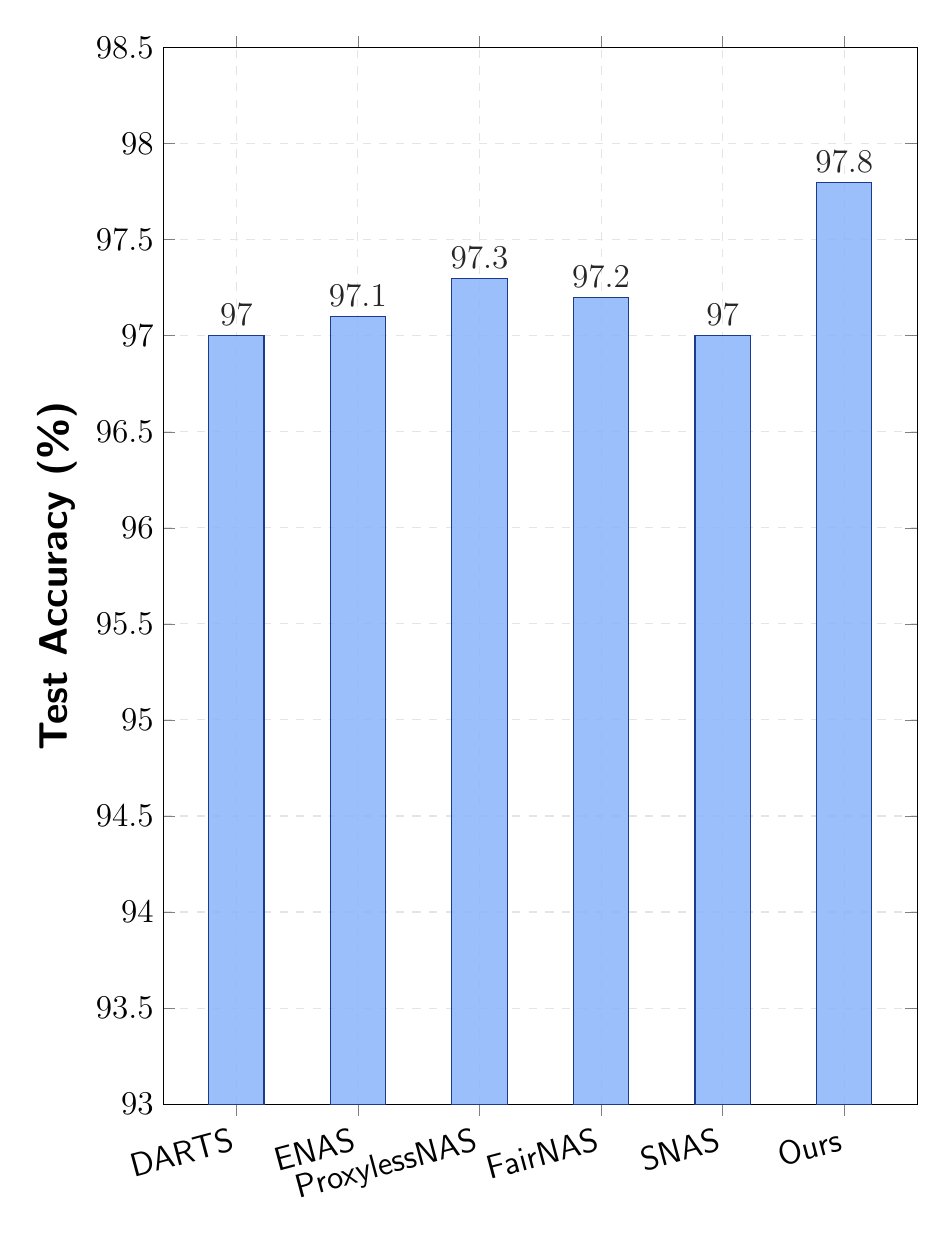
\begin{tikzpicture}
                \begin{axis}[
                    ybar,
                    bar width=20pt,
                    width=0.92\linewidth,
                    height=15cm,
                    ylabel={\textbf{Test Accuracy (\%)}},
                    ylabel style={font=\Large},
                    symbolic x coords={DARTS, ENAS, ProxylessNAS, FairNAS, SNAS, Ours},
                    xtick=data,
                    x tick label style={font=\large, rotate=15, anchor=north east},
                    y tick label style={font=\large},
                    ymin=93, ymax=98.5,
                    nodes near coords,
                    nodes near coords style={font=\large, /pgf/number format/fixed, /pgf/number format/precision=1},
                    enlarge x limits=0.12,
                    grid=major,
                    grid style={dashed, gray!20},
                    every axis plot/.append style={fill opacity=0.85}
                ]
                    \addplot[fill=steelblue!60, draw=navyblue] coordinates {
                        (DARTS, 97.0) (ENAS, 97.1) (ProxylessNAS, 97.3)
                        (FairNAS, 97.2) (SNAS, 97.0) (Ours, 97.8)
                    };
                \end{axis}
            \end{tikzpicture}
        \end{tikzfigure}

        \vspace{1em}

        % Results table
        \begin{center}
        {\large
        \begin{tabular}{lcccc}
            \toprule
            \textbf{Method} & \textbf{CIFAR-10} & \textbf{CIFAR-100} & \textbf{ImageNet Top-1} & \textbf{GPU Hours} \\
            \midrule
            DARTS           & 97.00\%  & 82.5\%  & 73.3\%  & 1.5   \\
            ENAS            & 97.11\%  & 83.1\%  & 74.0\%  & 0.5   \\
            ProxylessNAS    & 97.30\%  & 83.8\%  & 75.1\%  & 4.0   \\
            FairNAS         & 97.20\%  & 83.5\%  & 74.7\%  & 12.0  \\
            SNAS            & 97.02\%  & 82.9\%  & 73.9\%  & 1.5   \\
            \midrule
            \textbf{Ours}   & \textbf{97.82\%} & \textbf{85.3\%} & \textbf{76.4\%} & \textbf{0.4} \\
            \bottomrule
        \end{tabular}
        }
        \end{center}

        \vspace{1em}
        \coloredbox[bgcolor=navyblue!8, fgcolor=darktext, roundedcorners=5]{%
            \textbf{Highlight:} Our method achieves \textbf{state-of-the-art accuracy} (97.82\% CIFAR-10, 76.4\% ImageNet Top-1) with the \textbf{lowest search cost} (0.4 GPU hours --- 73\% less than DARTS).
        }
    }

    \block{Search Efficiency Analysis}{
        \begin{tikzfigure}[Search cost vs.\ accuracy trade-off. Circle size indicates model parameters (M).]
            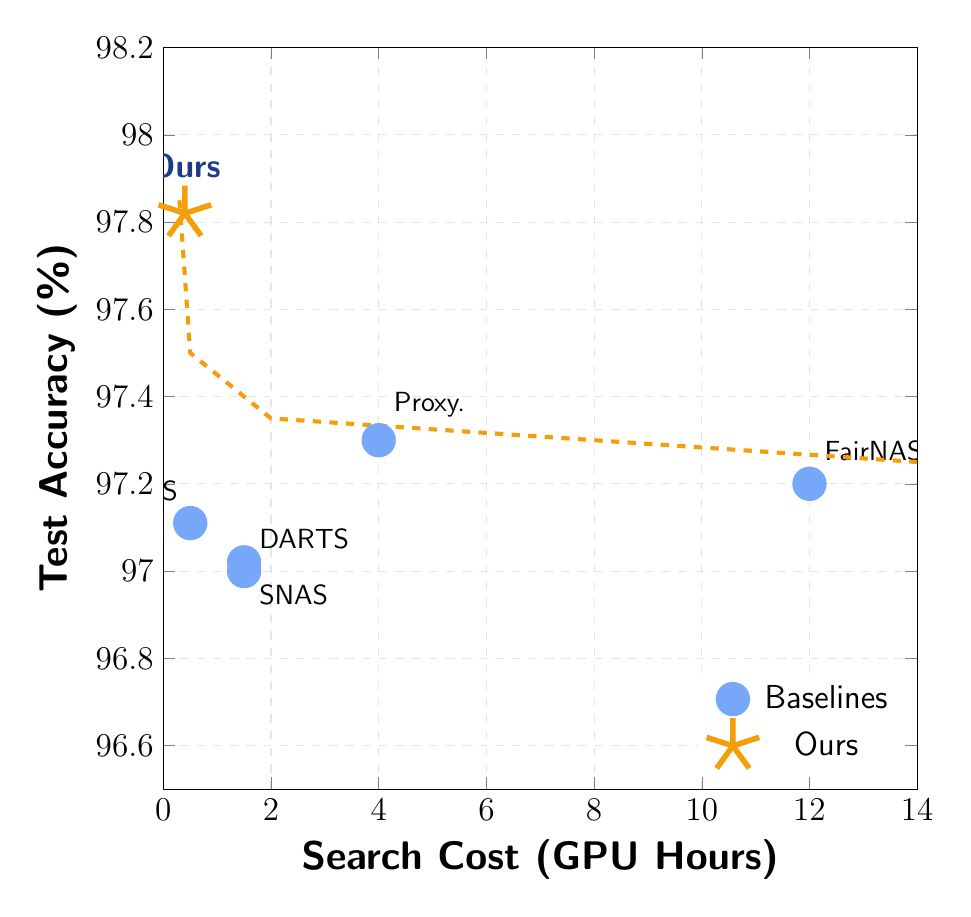
\begin{tikzpicture}
                \begin{axis}[
                    width=0.92\linewidth,
                    height=11cm,
                    xlabel={\textbf{Search Cost (GPU Hours)}},
                    ylabel={\textbf{Test Accuracy (\%)}},
                    xlabel style={font=\Large},
                    ylabel style={font=\Large},
                    x tick label style={font=\large},
                    y tick label style={font=\large},
                    xmin=0, xmax=14,
                    ymin=96.5, ymax=98.2,
                    grid=major,
                    grid style={dashed, gray!20},
                    legend style={at={(0.98,0.02)}, anchor=south east, font=\large, draw=none, fill=white!80}
                ]
                    \addplot[only marks, mark=*, mark size=6pt, color=steelblue!70] coordinates {
                        (1.5, 97.0) (0.5, 97.11) (4.0, 97.3) (12.0, 97.2) (1.5, 97.02)
                    };
                    \addlegendentry{Baselines}

                    \addplot[only marks, mark=star, mark size=10pt, color=amber, line width=2pt] coordinates {
                        (0.4, 97.82)
                    };
                    \addlegendentry{Ours}

                    \node[font=\normalsize, anchor=south west] at (axis cs:1.6, 97.03) {DARTS};
                    \node[font=\normalsize, anchor=south east] at (axis cs:0.45, 97.14) {ENAS};
                    \node[font=\normalsize, anchor=south west] at (axis cs:4.1, 97.33) {Proxy.};
                    \node[font=\normalsize, anchor=south west] at (axis cs:12.1, 97.23) {FairNAS};
                    \node[font=\normalsize, anchor=north west] at (axis cs:1.6, 96.99) {SNAS};
                    \node[font=\large, anchor=south, color=navyblue] at (axis cs:0.4, 97.88) {\textbf{Ours}};

                    \addplot[dashed, color=amber, line width=1.5pt, no markers] coordinates {
                        (0.3, 97.85) (0.5, 97.5) (2.0, 97.35) (14, 97.25)
                    };
                \end{axis}
            \end{tikzpicture}
        \end{tikzfigure}
    }

    \block{Conclusions \& Future Work}{
        We present \textbf{ENAS-Adaptive}, a gradient-based NAS method with adaptive resource allocation achieving state-of-the-art accuracy at a fraction of the search cost.

        \vspace{1em}
        \textbf{Key findings:}
        \begin{itemize}[leftmargin=*, itemsep=0.5em]
            \item 73\% faster search than DARTS with higher accuracy
            \item Architecture transfers well to ImageNet (+1.3\% over best baseline)
            \item Consistent across 3 datasets, 5 runs (std $<$ 0.1\%)
        \end{itemize}

        \vspace{1em}
        \textbf{Future:} Extend to detection/segmentation, hardware-aware objectives, larger search spaces.
    }

    \block{References \& Resources}{
        {\small
        [1] Liu et al. (2019). DARTS: Differentiable Architecture Search. \textit{ICLR}.

        [2] Pham et al. (2018). Efficient Neural Architecture Search. \textit{ICML}.

        [3] Cai et al. (2019). ProxylessNAS. \textit{ICLR}.
        }

        \vspace{1em}
        \begin{center}
        \qrcode[height=3.5cm]{https://github.com/achen/enas-adaptive}\\[0.5em]
        {\normalsize Paper \& Code}
        \end{center}

        \vspace{0.5em}
        {\small \textbf{Acknowledgments:} NSF Grant IIS-2024000 and Google Research Award.}
    }

\end{columns}

\end{document}
